% Options for packages loaded elsewhere
\PassOptionsToPackage{unicode}{hyperref}
\PassOptionsToPackage{hyphens}{url}
\documentclass[
  11pt,
  a4paper,
  fontset=none]{ctexart}
\usepackage{xcolor}
\usepackage[margin=22mm,headheight=15pt]{geometry}
\usepackage{amsmath,amssymb}
\setcounter{secnumdepth}{-\maxdimen} % remove section numbering
\usepackage{iftex}
\ifPDFTeX
  \usepackage[T1]{fontenc}
  \usepackage[utf8]{inputenc}
  \usepackage{textcomp} % provide euro and other symbols
\else % if luatex or xetex
  \usepackage{unicode-math} % this also loads fontspec
  \defaultfontfeatures{Scale=MatchLowercase}
  \defaultfontfeatures[\rmfamily]{Ligatures=TeX,Scale=1}
\fi
\usepackage{lmodern}
\ifPDFTeX\else
  % xetex/luatex font selection
\fi
% Use upquote if available, for straight quotes in verbatim environments
\IfFileExists{upquote.sty}{\usepackage{upquote}}{}
\IfFileExists{microtype.sty}{% use microtype if available
  \usepackage[]{microtype}
  \UseMicrotypeSet[protrusion]{basicmath} % disable protrusion for tt fonts
}{}
\makeatletter
\@ifundefined{KOMAClassName}{% if non-KOMA class
  \IfFileExists{parskip.sty}{%
    \usepackage{parskip}
  }{% else
    \setlength{\parindent}{0pt}
    \setlength{\parskip}{6pt plus 2pt minus 1pt}}
}{% if KOMA class
  \KOMAoptions{parskip=half}}
\makeatother
\usepackage{longtable,booktabs,array}
\usepackage{caption}
\captionsetup[table]{skip=6pt}
\newcounter{none} % for unnumbered tables
\usepackage{calc} % for calculating minipage widths
% Correct order of tables after \paragraph or \subparagraph
\usepackage{etoolbox}
\makeatletter
\patchcmd\longtable{\par}{\if@noskipsec\mbox{}\fi\par}{}{}
\makeatother
\usepackage{graphicx}
\makeatletter
\newsavebox\pandoc@box
\newcommand*\pandocbounded[1]{% scales image to fit in text height/width
  \sbox\pandoc@box{#1}%
  \Gscale@div\@tempa{\textheight}{\dimexpr\ht\pandoc@box+\dp\pandoc@box\relax}%
  \Gscale@div\@tempb{\linewidth}{\wd\pandoc@box}%
  \ifdim\@tempb\p@<\@tempa\p@\let\@tempa\@tempb\fi% select the smaller of both
  \ifdim\@tempa\p@<\p@\scalebox{\@tempa}{\usebox\pandoc@box}%
  \else\usebox{\pandoc@box}%
  \fi%
}
% Set default figure placement to htbp
\def\fps@figure{htbp}
\makeatother
\setlength{\emergencystretch}{3em} % prevent overfull lines
\providecommand{\tightlist}{%
  \setlength{\itemsep}{0pt}\setlength{\parskip}{0pt}}
% Scaling Law notes; style adapted from Attention/CN/pdf-header.tex.
\usepackage{fontspec}
\usepackage{enumitem}
\usepackage{fancyhdr}
\usepackage{fvextra}
\usepackage{etoolbox}

\setmainfont[
  Path=/usr/local/texlive/2026/texmf-dist/fonts/opentype/public/tex-gyre/,
  UprightFont=texgyrepagella-regular.otf,
  BoldFont=texgyrepagella-bold.otf,
  ItalicFont=texgyrepagella-italic.otf,
  BoldItalicFont=texgyrepagella-bolditalic.otf
]{texgyrepagella-regular.otf}
\setsansfont[
  Path=/usr/local/texlive/2026/texmf-dist/fonts/opentype/public/tex-gyre/,
  UprightFont=texgyreheros-regular.otf,
  BoldFont=texgyreheros-bold.otf,
  ItalicFont=texgyreheros-italic.otf,
  BoldItalicFont=texgyreheros-bolditalic.otf
]{texgyreheros-regular.otf}
\setmonofont[
  Path=/usr/local/texlive/2026/texmf-dist/fonts/opentype/google/roboto/,
  UprightFont=RobotoMono-Regular.otf,
  BoldFont=RobotoMono-Bold.otf,
  ItalicFont=RobotoMono-Italic.otf,
  BoldItalicFont=RobotoMono-BoldItalic.otf,
  Scale=0.82
]{RobotoMono-Regular.otf}
\setCJKmainfont[
  Path=/System/Library/Fonts/Supplemental/,
  FontIndex=6,
  BoldFont=Songti.ttc,
  BoldFeatures={FontIndex=1}
]{Songti.ttc}
\setCJKsansfont[
  Path=/System/Library/Fonts/,
  FontIndex=1,
  BoldFont={STHeiti Medium.ttc},
  BoldFeatures={FontIndex=1}
]{STHeiti Light.ttc}
\setCJKmonofont[Path=/System/Library/Fonts/,FontIndex=1]{STHeiti Light.ttc}

\definecolor{attentionblue}{HTML}{174A7E}
\definecolor{attentiongray}{HTML}{5D6773}
\definecolor{attentionlink}{HTML}{1769AA}
\definecolor{codebg}{HTML}{F4F6F8}

\AtBeginDocument{%
  \hypersetup{
    linkcolor=attentionblue,
    urlcolor=attentionlink,
    citecolor=attentionblue,
    pdftitle={Scaling Law：从算力分配到超参数预测}
  }%
}

\ctexset{
  section={format=\LARGE\bfseries\sffamily\color{attentionblue},beforeskip=1.8ex,afterskip=1.2ex},
  subsection={format=\Large\bfseries\sffamily\color{attentionblue},beforeskip=1.6ex,afterskip=0.9ex},
  subsubsection={format=\large\bfseries\sffamily\color{attentiongray},beforeskip=1.4ex,afterskip=0.7ex}
}

\setlength{\parindent}{2em}
\setlength{\parskip}{0.35em}
\linespread{1.18}
\setlist{itemsep=0.25em,topsep=0.45em,leftmargin=2.4em}
\setcounter{tocdepth}{2}
\setcounter{secnumdepth}{0}

\pagestyle{fancy}
\fancyhf{}
\fancyhead[L]{\small\sffamily\color{attentiongray} Scaling Law}
\fancyhead[R]{\small\sffamily\color{attentiongray} Purshow's Notes}
\fancyfoot[C]{\small\sffamily\thepage}
\renewcommand{\headrulewidth}{0.3pt}


\usepackage{caption}
\captionsetup{font=small,labelfont=bf}
\clearcaptionsetup{table} % The overview has no caption.
\usepackage{float}
\floatplacement{figure}{H}
\AtBeginDocument{\renewcommand{\figurename}{图}}

% A single opening page: article title above an automatically linked contents.
\makeatletter
\renewcommand*\l@subsection{\@dottedtocline{2}{0em}{0em}}
\renewcommand*\l@subsubsection{\@dottedtocline{3}{1.6em}{0em}}
\makeatother
\newcommand{\NotesCover}[1]{%
  \pagenumbering{roman}%
  \thispagestyle{empty}%
  \vspace*{0mm}%
  {\centering
    \sffamily\bfseries\color{attentionblue}%
    \fontsize{26pt}{36pt}\selectfont #1\par
  }%
  \vspace{4mm}%
  {\color{attentionblue}\noindent\rule{\linewidth}{0.6pt}\par}%
  \vspace{4mm}%
  \begingroup
    \setlength{\parindent}{0pt}%
    \setlength{\parskip}{0.6em}%
    \tableofcontents
  \endgroup
}
\newcommand{\NotesCoverEnd}{%
  \clearpage
  \pagenumbering{arabic}%
}

% Compact wrapping overview table, following Attention and MoE notes.
\newcommand{\OverviewTableStyle}{%
  \linespread{1}\fontsize{8.5pt}{10.5pt}\selectfont
  \setlength{\tabcolsep}{2.5pt}%
  \renewcommand{\arraystretch}{1.15}%
  \setlength{\extrarowheight}{6pt}%
  \setlength{\LTpre}{22pt}%
  \setlength{\LTpost}{0pt}%
  \setlength{\parskip}{0pt}%
}

% Keep the compact lookup flow together on one page.
\BeforeBeginEnvironment{verbatim}{\begin{samepage}}
\AfterEndEnvironment{verbatim}{\end{samepage}}

% Avoid isolated first or last lines at page boundaries.
\clubpenalty=10000
\widowpenalty=10000
\displaywidowpenalty=10000

% An unbreakable formula group keeps the introduction and display together.
\newenvironment{NotesFormula}{%
  \par\noindent\begin{minipage}{\linewidth}%
  \setlength{\parindent}{2em}%
  \setlength{\parskip}{0.35em}%
}{\end{minipage}\par}
\usepackage{bookmark}
\IfFileExists{xurl.sty}{\usepackage{xurl}}{} % add URL line breaks if available
\urlstyle{same}
% fallback for those not using the hyperref driver hyperxmp:
\makeatletter
\@ifundefined{xmpquote}{\newcommand{\xmpquote}[1]{#1}}{}
\makeatother
\hypersetup{
  hidelinks,
  pdfcreator={LaTeX via pandoc}}

\author{}
\date{}

\begin{document}

\NotesCover{Scaling Law：从算力分配到超参数预测}

\begingroup\OverviewTableStyle

{\def\LTcaptype{none} % do not increment counter
\begin{longtable}[]{@{}
  >{\centering\arraybackslash}p{(\linewidth - 6\tabcolsep) * \real{0.2000}}
  >{\centering\arraybackslash}p{(\linewidth - 6\tabcolsep) * \real{0.2400}}
  >{\centering\arraybackslash}p{(\linewidth - 6\tabcolsep) * \real{0.2700}}
  >{\centering\arraybackslash}p{(\linewidth - 6\tabcolsep) * \real{0.2900}}@{}}
\toprule\noalign{}
\begin{minipage}[b]{\linewidth}\centering
\textbf{工作}
\end{minipage} & \begin{minipage}[b]{\linewidth}\centering
\textbf{时间}
\end{minipage} & \begin{minipage}[b]{\linewidth}\centering
\textbf{研究问题}
\end{minipage} & \begin{minipage}[b]{\linewidth}\centering
\textbf{核心方法}
\end{minipage} \\
\midrule\noalign{}
\endhead
\bottomrule\noalign{}
\endlastfoot
\textbf{Rosenfeld et al.} & 2019.09 & 误差如何随 \(N,D\) 联合变化 &
多架构 / 优化器下的联合幂律拟合 \\
\textbf{Kaplan Law} & 2020.01 & Loss 如何随 \(N,D,C\) 变化 & 幂律拟合 +
Critical Batch Size 校正 \\
\textbf{Chinchilla~Law} & 2022.03 & 固定 \(C\) 如何分配 \(N,D\) &
Envelope / IsoFLOP / Parametric Fit \\
\textbf{DeepSeek Law} & 2024.01 & 改进算力定义 + 超参数随 \(C\) 变化 &
Non-Embedding FLOPs/token \(M\) + IsoFLOP \\
\textbf{Microsoft Law} & 2024.09 & 最优 LR 如何随 \(N,D\) 变化 & LR
Sweep + 二次拟合 + 幂律拟合 \\
\textbf{Step Law} & 2025.03 & 直接预测最优 LR 与 BS & 3,700+ 模型 Grid
Search + OLS + Bootstrap \\
\textbf{Farseer} & 2025.06 & \(N,D\) 的交互项 & Differential Piecewise
Fitting \\
\textbf{MAI} & 2026.10 & 小模型实验如何可靠迁移到大模型 & Scaling Ladder
+ 固定 TPP + Source Scaling \\
\end{longtable}
}

\endgroup

\NotesCoverEnd

\subsection{零、什么是 Scaling
Law}\label{ux96f6ux4ec0ux4e48ux662f-scaling-law}

我们先给出一些有用的概念与常见的结论。

Scaling Law
的概念是：随着模型规模、数据集规模以及计算资源的增加，训练损失会以可预测的方式下降。这种下降趋势遵循幂律曲线，而在对数坐标图中则表现为一条直线。我们可以将
Scaling Law
视为描述计算资源、损失、模型规模和数据之间关系的框架。其核心在于如何合理分配宝贵的计算资源，以便在各种因素之间取得最佳平衡。

\subsubsection{符号约定}\label{ux7b26ux53f7ux7ea6ux5b9a}

\(N\) 为模型参数量；\(D\) 为训练 Token 数；\(C\)
为训练计算量（FLOPs）；\(E\) 为不可约 Loss；\(L,\hat L(\cdot)\) 为测试
Loss 及其预测函数（也可指训练 Loss，两者强相关）；\(\epsilon\)
为泛化误差。

\subsubsection{\texorpdfstring{\(常见的C\approx6ND\)
是怎么来的？}{常见的C\textbackslash approx6ND 是怎么来的？}}\label{ux5e38ux89c1ux7684capprox6nd-ux662fux600eux4e48ux6765ux7684}

Transformer 的计算几乎都是矩阵乘，而一个 Token 经过权重矩阵
\(W\in\mathbb R^{d_{\mathrm{in}}\times d_{\mathrm{out}}}\) 的开销是
\(2d_{\mathrm{in}}d_{\mathrm{out}}\) FLOPs，即\textbf{每个参数一次乘加 =
2 FLOPs}：

\begin{itemize}
\tightlist
\item
  \textbf{前向}：\(Y=XW\)，每 Token \(2N\)；
\item
  \textbf{反向}：\(\partial\mathcal L/\partial X=GW^\top\)（传给前一层）与
  \(\partial\mathcal L/\partial W=X^\top G\)（更新参数）两次同规模矩阵乘，每
  Token \(4N\)。
\end{itemize}

\[C\approx\underbrace{2ND}_{\text{forward}}+\underbrace{4ND}_{\text{backward}}=6ND.\]

当然这肯定是省略了一些计算的：

\begin{itemize}
\tightlist
\item
  \textbf{Attention 的 \(QK^\top\)、\(AV\)}：每层每 Token 前向约
  \(4Sd\)（\(S\) 为上下文长度），与权重项之比约
  \(S/6d\)，长上下文时不可忽略；DeepSeek 的 \(M=72Ld^2+12LdS\)
  就是把它算进来的版本。
\item
  \textbf{Embedding、Norm、Softmax、激活、残差}：查表或 \(O(d)\)
  逐元素运算，相比 \(O(d^2)\) 可忽略。
\item
  \textbf{优化器更新}：每 Step 一次而非每 Token 一次，摊销后可忽略。
\end{itemize}

\subsubsection{为什么我们喜欢幂律？}\label{ux4e3aux4ec0ux4e48ux6211ux4eecux559cux6b22ux5e42ux5f8b}

\begin{NotesFormula}

因为取对数之后：

\[\log L=\log A-\alpha\log N\]

\end{NotesFormula}

就会变成一条直线。

这意味着我们可以在较小模型上拟合直线，进而预测更大模型的
Loss。\textbf{幂律使 Scaling Law
能够通过简单的回归拟合得到参数，从而进行外推；但外推是否准确，取决于幂律在更大规模上是否仍然成立。}

\subsubsection{\texorpdfstring{Rosenfeld：\(N\) 与 \(D\)
的联合函数}{Rosenfeld：N 与 D 的联合函数}}\label{rosenfeldn-ux4e0e-d-ux7684ux8054ux5408ux51fdux6570}

\begin{NotesFormula}

\href{https://arxiv.org/abs/1909.12673}{A Constructive Prediction of the
Generalization Error Across Scales}（Rosenfeld et
al.~2020）进一步研究了这一问题。他们试图将误差视为模型规模 \(N\)
和数据规模 \(D\)
的联合函数，同时考察了多种架构（ResNet、WRN、LSTM、Transformer）以及优化器（Adam、SGD
的各类变体）对误差的影响。实证结果表明：在固定其中一个变量的情况下，误差会以另一个变量的幂律形式衰减：

\[\hat L(D,N)\approx\frac{A}{N^\alpha}+E_N,\qquad
\hat L(D,N)\approx\frac{B}{D^\beta}+E_D.\]

\end{NotesFormula}

\begin{NotesFormula}

这些可以组合成一种联合形式：

\[\boxed{\hat L(N,D)=E+\frac{A}{N^\alpha}+\frac{B}{D^\beta}}\]

\end{NotesFormula}

其中 \(A>0,B>0,\alpha\ge0,\beta\ge0\) 为标量常数，而 \(E\) 的值与 \(N\)
和 \(D\) 均无关。它包含三项：

{\def\LTcaptype{none} % do not increment counter
\begin{longtable}[]{@{}cl@{}}
\toprule\noalign{}
\textbf{项} & \textbf{意义} \\
\midrule\noalign{}
\endhead
\bottomrule\noalign{}
\endlastfoot
\(A/N^\alpha\) & 模型容量不足引起的 Loss \\
\(B/D^\beta\) & 训练数据不足引起的 Loss \\
\(E\) & 不可约 Loss \\
\end{longtable}
}

\clearpage

\subsection{一、Kaplan et al.'s Scaling
Laws}\label{ux4e00kaplan-et-al.s-scaling-laws}

\href{https://arxiv.org/abs/2001.08361}{Scaling Laws for Neural Language
Models}（Kaplan et al.~2020）在语言模型领域推广了 Scaling Law
这一概念。他们发现，交叉熵测试 Loss \(L\) 与模型规模 \(N\)（不包括
Embedding 层）、数据集规模 \(D\) 以及训练计算量 \(C\)
之间的关系均符合幂律，并且在多个数量级上都成立。这些发现与上一节中的早期研究一致，不过
Kaplan 等人以 Transformer
语言模型为研究对象，进行了更大规模的实证实验：模型规模从 768 到 1.5B 非
Embedding 参数（当然，今日来看已然不大），数据集规模从 22M 到 23B
Tokens。论文中所有训练都采用相同的学习率调度：先进行 3000 步线性
Warmup，之后余弦衰减至零。

{\def\LTcaptype{none} % do not increment counter
\begin{longtable}[]{@{}
  >{\centering\arraybackslash}p{(\linewidth - 4\tabcolsep) * \real{0.2185}}
  >{\centering\arraybackslash}p{(\linewidth - 4\tabcolsep) * \real{0.3613}}
  >{\centering\arraybackslash}p{(\linewidth - 4\tabcolsep) * \real{0.4202}}@{}}
\toprule\noalign{}
\begin{minipage}[b]{\linewidth}\centering
\textbf{研究方向}
\end{minipage} & \begin{minipage}[b]{\linewidth}\centering
\textbf{核心问题}
\end{minipage} & \begin{minipage}[b]{\linewidth}\centering
\textbf{主要结论}
\end{minipage} \\
\midrule\noalign{}
\endhead
\bottomrule\noalign{}
\endlastfoot
1. Model Scaling & 参数量 \(N\) 如何影响 Loss？ &
\(L(N)\propto N^{-0.076}\) \\
2. Data Scaling & 数据量 \(D\) 如何影响 Loss？ &
\(L(D)\propto D^{-0.095}\) \\
3. Compute Scaling & 计算量 \(C\) 如何影响 Loss？ &
\(L(C_{\min})\propto C_{\min}^{-0.050}\) \\
4. Model Shape & Depth、Width、Heads 等结构参数有多重要？ &
固定参数量时，合理范围内影响较小 \\
5. Overfitting & 参数量与数据量如何共同决定 Loss？ & 过拟合惩罚主要与
\(N^{0.74}/D\) 有关 \\
6. Training Dynamics & Loss 如何随训练步数下降？ & 拟合
\(L(N,S_{\min})\)，并研究 Critical Batch Size \\
7. Compute-Optimal Scaling & 固定 FLOPs，应该如何分配参数量和 Token 数？
& \(N^*\propto C^{0.73}\)，\(D^*\propto C^{0.27}\) \\
\end{longtable}
}

\subsubsection{\texorpdfstring{联合 Loss 函数
\(L(N,D)\)}{联合 Loss 函数 L(N,D)}}\label{ux8054ux5408-loss-ux51fdux6570-lnd}

\begin{NotesFormula}

单独研究 \(N\) 和 \(D\) 还不够，因为实际训练中两者会同时影响
Loss。Kaplan 在 Section 4 中提出：

\[\boxed{L(N,D)=\left[\left(\frac{N_c}{N}\right)^{\alpha_N/\alpha_D}+\frac{D_c}{D}\right]^{\alpha_D}}\]

\end{NotesFormula}

它描述了模型容量和数据规模共同决定的 Loss 下界。这里有两个重要结论：

\begin{itemize}
\tightlist
\item
  当 \(D\to\infty\)，Loss 主要由参数量 \(N\) 决定。
\item
  当 \(N\to\infty\)，Loss 主要由数据量 \(D\) 决定。
\end{itemize}

\begin{NotesFormula}

实验还发现，为控制过拟合带来的相对 Loss 惩罚，数据规模大致需要满足：

\[D\propto N^{0.74}\]

\end{NotesFormula}

\subsubsection{Critical Batch Size}\label{critical-batch-size}

Batch Size 决定了训练的两种成本：\textbf{训练步数}（Wall-clock
时间）与\textbf{处理的 Tokens 数}（计算量）。Kaplan Law 借用 McCandlish
et al.（2018）的经验关系来刻画二者的权衡，并由此定义 Critical Batch
Size。

\begin{NotesFormula}

\textbf{1. 经验关系。} 训练模型达到相同 Loss 时，训练步数与处理的 Tokens
数之间存在近似固定的权衡：

\[\boxed{\left(\frac{S}{S_{\min}}-1\right)\left(\frac{E}{E_{\min}}-1\right)=1}\]

\end{NotesFormula}

其中 \(S\) 为达到目标 Loss 所需的训练步数，\(S_{\min}\)
为理论最少步数（Batch 无限大时）；\(E=BS\) 为累计处理的
Tokens，\(E_{\min}\) 为理论最少 Tokens（Batch 无限小时）。

\begin{NotesFormula}

\textbf{2. 小 Batch 与大 Batch 的权衡。} 代入 \(E=BS\)，可将上式整理为：

\[\boxed{S=S_{\min}+\frac{E_{\min}}{B}},\qquad
\boxed{E=E_{\min}+BS_{\min}}\]

\end{NotesFormula}

\begin{itemize}
\tightlist
\item
  小 Batch：梯度噪声较大，训练步数多，但 Token 利用效率高，\(E\) 接近
  \(E_{\min}\)。
\item
  大 Batch：梯度噪声较小，训练步数少（\(S\) 接近
  \(S_{\min}\)），但存在边际收益递减，处理更多 Tokens
  却无法显著减少步数。
\end{itemize}

即 \textbf{小 Batch 计算效率高，大 Batch 训练步数效率高}，又是
tradeoff。

\begin{NotesFormula}

\textbf{3. 定义 Critical Batch Size。} 为找到两种效率之间的平衡点，令
\(S=S_{\min}+E_{\min}/B\) 中两项相等，\(S_{\min}=E_{\min}/B\)，得到：

\[\boxed{B_{\mathrm{crit}}=\frac{E_{\min}}{S_{\min}}}\]

\end{NotesFormula}

此时
\(S=2S_{\min}\)，\(E=2E_{\min}\)------步数和计算量都只比各自的理论最优多一倍。由此：

\begin{itemize}
\tightlist
\item
  \(B\ll B_{\mathrm{crit}}\)：增大 Batch
  能显著减少训练步数，且几乎不增加计算量。
\item
  \(B\gg B_{\mathrm{crit}}\)：继续增大 Batch 的收益很小，计算浪费明显。
\end{itemize}

\begin{NotesFormula}

\textbf{4. \(B_{\mathrm{crit}}\) 与 Loss 的关系。} Kaplan 通过不同 Batch
Size 的训练实验拟合：

\[\boxed{B_{\mathrm{crit}}(L)\propto L^{-4.76}}\]

\end{NotesFormula}

即 \textbf{Loss 越低，Critical Batch Size
越大}：训练越往后，梯度信号越弱、噪声相对越大，需要更大的 Batch
才能有效估计梯度。

\subsubsection{如何研究 Compute-Optimal Scaling
Law？}\label{ux5982ux4f55ux7814ux7a76-compute-optimal-scaling-law}

目标：给定计算预算 \(C\)，如何分配模型规模、Batch Size 和训练步数，让
Loss 最小？研究步骤：

\begin{enumerate}
\def\labelenumi{\arabic{enumi}.}
\tightlist
\item
  \textbf{校正 Batch Size 效率}：利用
  \(B_{\mathrm{crit}}\)，把实际计算量和训练步数转换为理想最小值。
\end{enumerate}

\[S_{\min}=\frac{S}{1+B_{\mathrm{crit}}/B},\qquad
C_{\min}=\frac{C}{1+B/B_{\mathrm{crit}}}\]

\begin{enumerate}
\def\labelenumi{\arabic{enumi}.}
\setcounter{enumi}{1}
\tightlist
\item
  \textbf{拟合训练曲线}：研究不同模型规模和训练步数对应的 Loss。
\end{enumerate}

\[\boxed{L(N,S_{\min})=\left(\frac{N_c}{N}\right)^{\alpha_N}+\left(\frac{S_c}{S_{\min}}\right)^{\alpha_S}}\]

\begin{enumerate}
\def\labelenumi{\arabic{enumi}.}
\setcounter{enumi}{2}
\tightlist
\item
  \textbf{固定计算预算，寻找最优模型规模}：
\end{enumerate}

\[\min_{N,S_{\min}}L(N,S_{\min})\qquad
\text{s.t.}\quad C_{\min}=6NB_{\mathrm{crit}}(L)S_{\min}\]

\begin{NotesFormula}

通过优化联合函数，并对不同预算下的最优实验结果进行拟合，得到：

\[\boxed{
\begin{aligned}
N_{\mathrm{opt}}&\propto C_{\min}^{0.73}\\
B_{\mathrm{crit}}&\propto C_{\min}^{0.24}\\
S_{\min}&\propto C_{\min}^{0.03}
\end{aligned}}\]

\end{NotesFormula}

结论：Kaplan
认为增加训练算力时，应该\textbf{主要用于扩大模型规模}，而不是显著增加训练步数；最优训练应在模型完全收敛之前停止。（因此我们可以看到21年左右的模型近乎畸形的大）

以上是 Kaplan（2020）的经典原始结论，后续
Chinchilla（2022）修正了最优模型规模与训练 Tokens 的增长比例。

\clearpage

\subsection{二、Chinchilla}\label{ux4e8cchinchilla}

\href{https://arxiv.org/abs/2203.15556}{Training Compute-Optimal Large
Language Models}（Hoffmann et al.~2022）认为 Kaplan 存在两个问题：

\begin{enumerate}
\def\labelenumi{\arabic{enumi}.}
\tightlist
\item
  \textbf{Learning Rate Schedule 的问题。} Kaplan
  的部分分析依赖固定训练长度对应的 LR Schedule，并使用训练过程中的中间
  Loss 预测较短训练时长的表现。但当目标训练 Tokens
  较少时，若学习率仍按较长的训练周期衰减，那么在中间检查点学习率尚未充分降低，Loss
  可能偏高，从而影响 Compute-Optimal 的估计。
\item
  \textbf{模型规模偏小的问题。} Kaplan 的实验包含大量不足 100M
  参数的模型，而 Chinchilla 将 Scaling 实验扩大到约 70M--16B
  参数，并观察到最优 Scaling
  曲线可能存在一定曲率。因此，仅使用小模型进行外推可能产生偏差。
\end{enumerate}

\begin{NotesFormula}

研究问题：给定固定的训练计算预算 \(C\)，应该使用多少模型参数
\(N\)，以及训练多少 Tokens \(D\)，才能获得最低的最终预训练 Loss？

\[\boxed{(N_{\mathrm{opt}},D_{\mathrm{opt}})=\mathop{\mathrm{argmin}}_{N,D}\,L(N,D)\quad\text{s.t.}\quad 6ND=C}\]

\end{NotesFormula}

固定 \(C\) 后，模型规模与训练 Tokens 之间必然存在权衡
\(D=C/(6N)\)：模型越大，可用于训练的 Tokens 就越少。Chinchilla
用三种方法回答这一问题。

\subsubsection{1. Training Curve
Envelope（训练曲线包络线）}\label{training-curve-envelopeux8badux7ec3ux66f2ux7ebfux5305ux7edcux7ebf}

\begin{enumerate}
\def\labelenumi{\arabic{enumi}.}
\tightlist
\item
  训练不同参数量的模型，记录 Loss 随 FLOPs 变化的曲线。
\item
  对每个计算预算 \(C\)，找到 Loss 最低的模型配置。
\item
  拟合最优参数量和 Tokens 随计算量的变化关系。
\end{enumerate}

\begin{NotesFormula}

结论：

\[N_{\mathrm{opt}}\propto C^{0.50},\qquad D_{\mathrm{opt}}\propto C^{0.50}\]

\end{NotesFormula}

\begin{center}

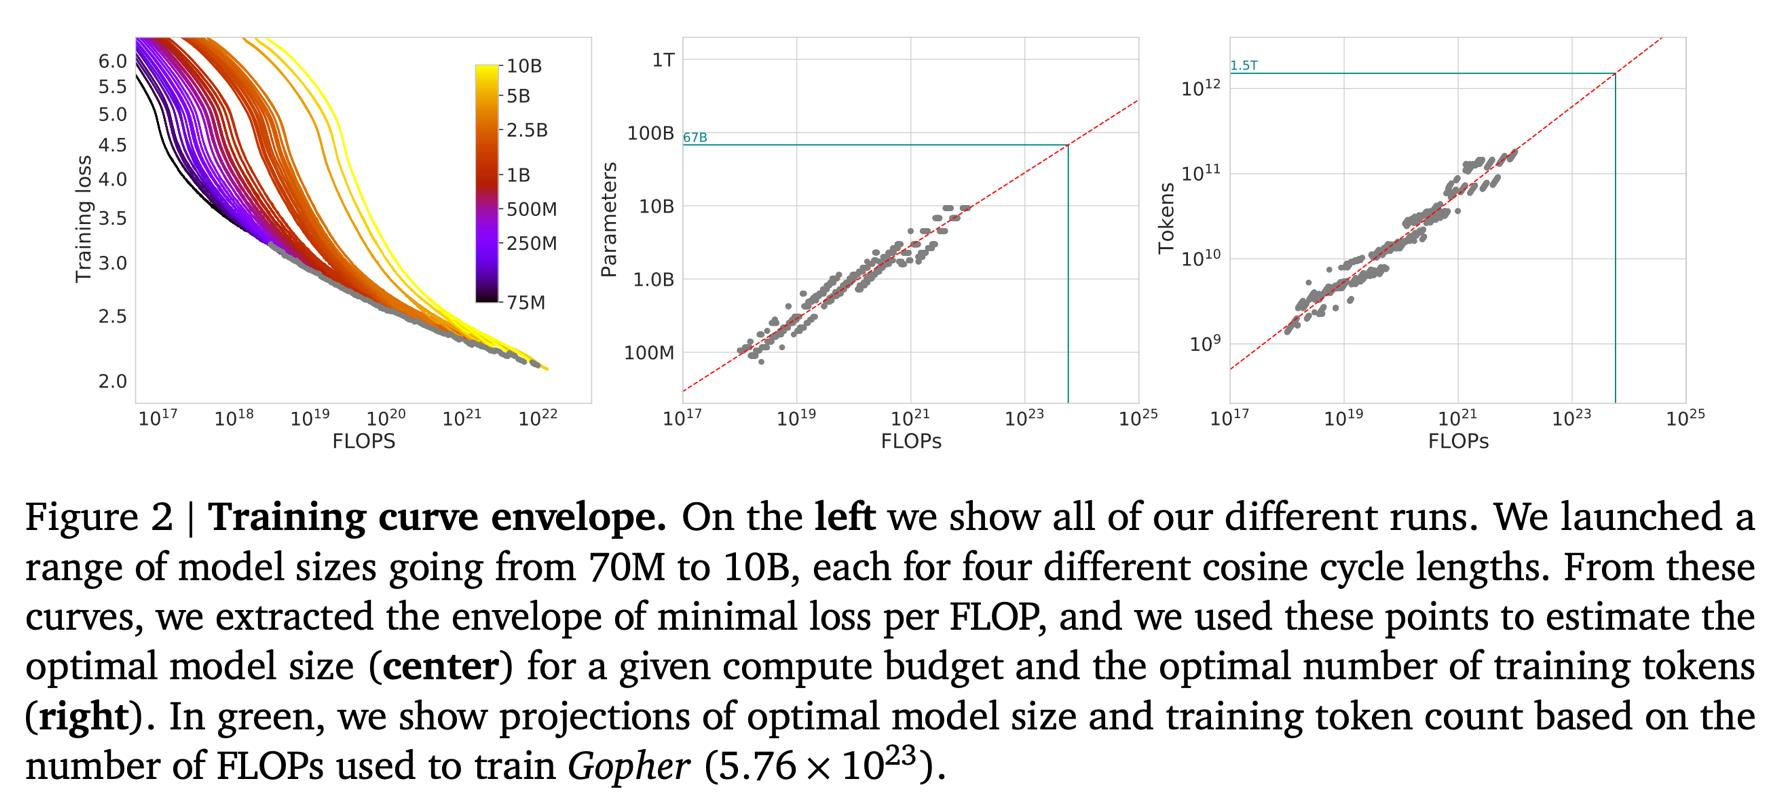
\includegraphics[width=0.72\linewidth,height=\textheight,keepaspectratio,alt={Chinchilla
Approach 1：Training Curve Envelope}]{assets/chinchilla-envelope.png}

\end{center}

\clearpage

\subsubsection{2.
IsoFLOP（固定计算量实验）}\label{isoflopux56faux5b9aux8ba1ux7b97ux91cfux5b9eux9a8c}

\begin{enumerate}
\def\labelenumi{\arabic{enumi}.}
\tightlist
\item
  \textbf{固定计算预算 \(C\)}：改变模型参数量 \(N\)，同时令训练 Tokens
  \(D=C/(6N)\)。
\item
  \textbf{寻找最优配置}：训练所有配置并记录最终
  Loss，对实验点做二次曲线拟合，最低点即 \(N_{\mathrm{opt}}\)，并得到
  \(D_{\mathrm{opt}}=C/(6N_{\mathrm{opt}})\)。
\item
  \textbf{拟合 Scaling Law}：对多个 \(C\) 重复实验，得到多组
  \((C,N_{\mathrm{opt}},D_{\mathrm{opt}})\)，再做幂律拟合。
\end{enumerate}

\begin{NotesFormula}

结论：

\[\boxed{N_{\mathrm{opt}}\propto C^{0.49},\qquad D_{\mathrm{opt}}\propto C^{0.51}}\]

\end{NotesFormula}

核心：\textbf{两次拟合}------先用二次曲线寻找固定 FLOPs
下的最优配置，再用幂律拟合最优配置与 FLOPs 的关系。

\begin{center}

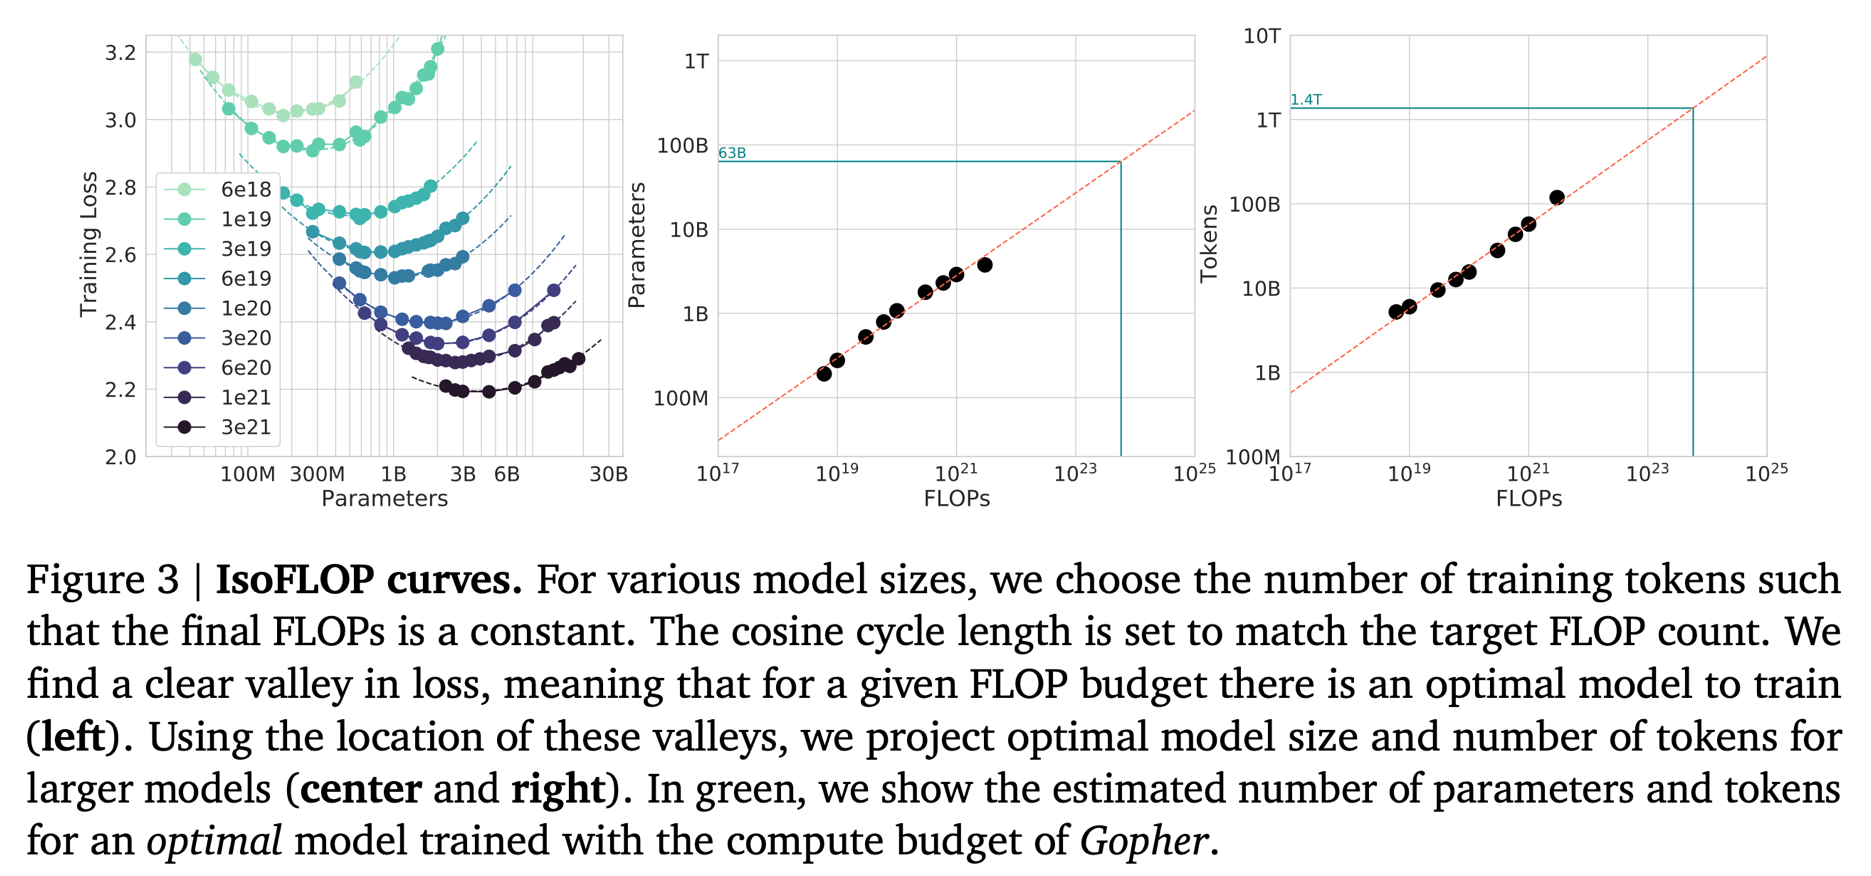
\includegraphics[width=0.72\linewidth,height=\textheight,keepaspectratio,alt={Chinchilla
Approach 2：IsoFLOP Curves}]{assets/chinchilla-isoflop.png}

\end{center}

\subsubsection{3. Parametric Loss Function（参数化 Loss
拟合）}\label{parametric-loss-functionux53c2ux6570ux5316-loss-ux62dfux5408}

\begin{center}

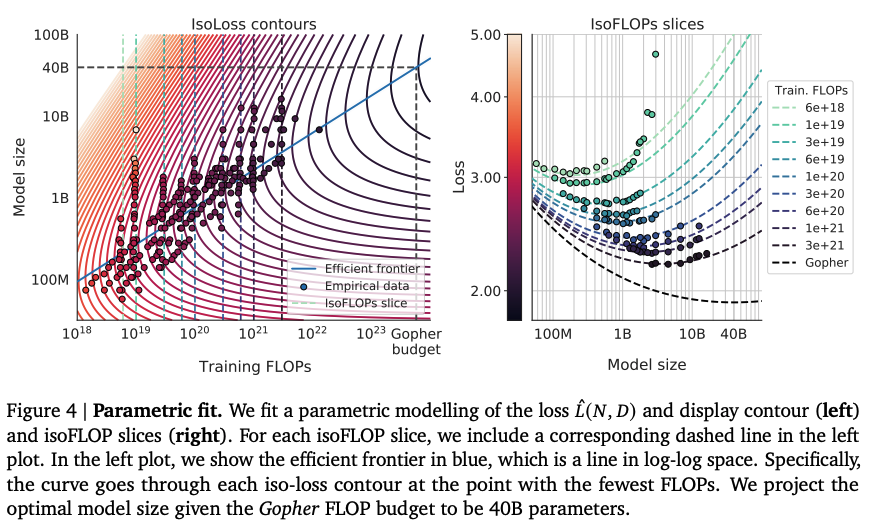
\includegraphics[width=0.8\linewidth,height=\textheight,keepaspectratio,alt={Chinchilla
Approach 3：Parametric Fit}]{assets/chinchilla-parametric.png}

\end{center}

\begin{enumerate}
\def\labelenumi{\arabic{enumi}.}
\tightlist
\item
  \textbf{收集实验数据}：利用前两种方法训练的模型，收集不同参数量
  \(N\)、训练 Tokens \(D\) 对应的最终 Training Loss，得到数据点
  \((N_i,D_i,L_i)\)。
\item
  \textbf{拟合 Loss 函数}：假设 Loss 满足：
\end{enumerate}

\[L(N,D)=E+\frac{A}{N^\alpha}+\frac{B}{D^\beta}\]

\begin{NotesFormula}

其中，\(E\) 是不可约
Loss，后两项分别描述模型规模和训练数据量有限带来的误差。使用 Huber Loss
+ L-BFGS 拟合 \(A,B,E,\alpha,\beta\)：

\[\min_{\theta}\sum_i\operatorname{Huber}_{10^{-3}}\left(\log\hat L(N_i,D_i;\theta)-\log L_i\right)\]

\end{NotesFormula}

其中 \(\theta=(A,B,E,\alpha,\beta)\)。

\begin{enumerate}
\def\labelenumi{\arabic{enumi}.}
\setcounter{enumi}{2}
\tightlist
\item
  \textbf{求解最优算力分配}：固定计算预算 \(C=6ND\)，将 \(D=C/(6N)\)
  代入拟合的 Loss 函数：
\end{enumerate}

\[L(N)=E+\frac{A}{N^\alpha}+B\left(\frac{6N}{C}\right)^\beta\]

\begin{NotesFormula}

对 \(N\) 求导，令 \(\frac{dL}{dN}=0\)，得到：

\[N_{\mathrm{opt}}\propto C^{\frac{\beta}{\alpha+\beta}},\qquad
D_{\mathrm{opt}}\propto C^{\frac{\alpha}{\alpha+\beta}}\]

\end{NotesFormula}

\begin{NotesFormula}

结论：原论文拟合得到
\(\alpha\approx0.34,\beta\approx0.28\)，使用未舍入参数计算：

\[\boxed{N_{\mathrm{opt}}\propto C^{0.46},\qquad D_{\mathrm{opt}}\propto C^{0.54}}\]

\end{NotesFormula}

\subsubsection{三种方法的核心区别}\label{ux4e09ux79cdux65b9ux6cd5ux7684ux6838ux5fc3ux533aux522b}

\begin{NotesFormula}

Tokens per Parameter 定义为：

\[\boxed{R=\frac{D_{\mathrm{opt}}}{N_{\mathrm{opt}}}}\]

\end{NotesFormula}

下表以 \emph{Gopher} 的计算预算（\(5.76\times10^{23}\) FLOPs，对应
Approach 1 的 67B
最优模型）为例，比较不同方法推荐的最优模型规模、训练数据量及比例（数值取自上面三张图中的
Gopher 投影）。

{\def\LTcaptype{none} % do not increment counter
\begin{longtable}[]{@{}
  >{\centering\arraybackslash}p{(\linewidth - 10\tabcolsep) * \real{0.1350}}
  >{\centering\arraybackslash}p{(\linewidth - 10\tabcolsep) * \real{0.2025}}
  >{\centering\arraybackslash}p{(\linewidth - 10\tabcolsep) * \real{0.2025}}
  >{\centering\arraybackslash}p{(\linewidth - 10\tabcolsep) * \real{0.1840}}
  >{\centering\arraybackslash}p{(\linewidth - 10\tabcolsep) * \real{0.1840}}
  >{\centering\arraybackslash}p{(\linewidth - 10\tabcolsep) * \real{0.0920}}@{}}
\toprule\noalign{}
\begin{minipage}[b]{\linewidth}\centering
\textbf{方法}
\end{minipage} & \begin{minipage}[b]{\linewidth}\centering
\(N_{\mathrm{opt}}\propto C^{a}\)
\end{minipage} & \begin{minipage}[b]{\linewidth}\centering
\(D_{\mathrm{opt}}\propto C^{b}\)
\end{minipage} & \begin{minipage}[b]{\linewidth}\centering
\textbf{\(N_{\mathrm{opt}}\)}
\end{minipage} & \begin{minipage}[b]{\linewidth}\centering
\textbf{\(D_{\mathrm{opt}}\)}
\end{minipage} & \begin{minipage}[b]{\linewidth}\centering
\textbf{\(R\)}
\end{minipage} \\
\midrule\noalign{}
\endhead
\bottomrule\noalign{}
\endlastfoot
Approach 1：Envelope & 0.50 & 0.50 & 67B & 1.5T & \(\approx22\) \\
Approach 2：IsoFLOP & 0.49 & 0.51 & 63B & 1.4T & \(\approx22\) \\
Approach 3：Parametric & 0.46 & 0.54 & 40B & \(\approx2.4\)T &
\(\approx60\) \\
Kaplan (2020) & 0.73 & 0.27 & - & - & - \\
\end{longtable}
}

注：Approach 3 的 \(D_{\mathrm{opt}}\) 由 \(C/(6N_{\mathrm{opt}})\)
推得。

有趣的是，后面 \href{https://arxiv.org/abs/2404.10102}{Chinchilla
Scaling: A replication attempt} 利用 Chinchilla
论文图表重建训练数据，重新使用 Huber Loss 拟合 Parametric Loss
Function，发现原论文存在\textbf{优化器提前停止}、\textbf{参数精度问题（四舍五入两位小数害了它）}，以及
\textbf{Scaling 指数置信区间过窄}等问题。修正后的 Scaling 指数分别为
\(0.513\) 和 \(0.487\)，与前两种方法更加一致。

\subsubsection{Kaplan vs.~Chinchilla}\label{kaplan-vs.-chinchilla}

为什么两者的结论会有这么大的区别呢？

\begin{enumerate}
\def\labelenumi{\arabic{enumi}.}
\tightlist
\item
  \textbf{Kaplan 模型小}：大量实验点落在不足 100M 参数的区间，而最优
  Scaling 曲线存在曲率，小模型区间的斜率外推到大规模会产生偏差。
\item
  \textbf{Embedding parameter count matters for small models.} Kaplan
  使用非 Embedding 参数量，Chinchilla
  使用总参数量。对小模型而言，Embedding
  在总参数中占比很高，两种计数方式会显著改变小模型区间的拟合斜率；而模型越大，这一差异越小。
\end{enumerate}

{\def\LTcaptype{none} % do not increment counter
\begin{longtable}[]{@{}
  >{\centering\arraybackslash}p{(\linewidth - 4\tabcolsep) * \real{0.2105}}
  >{\centering\arraybackslash}p{(\linewidth - 4\tabcolsep) * \real{0.3684}}
  >{\centering\arraybackslash}p{(\linewidth - 4\tabcolsep) * \real{0.4211}}@{}}
\toprule\noalign{}
\begin{minipage}[b]{\linewidth}\centering
\end{minipage} & \begin{minipage}[b]{\linewidth}\centering
\textbf{Kaplan (2020)}
\end{minipage} & \begin{minipage}[b]{\linewidth}\centering
\textbf{Chinchilla (2022)}
\end{minipage} \\
\midrule\noalign{}
\endhead
\bottomrule\noalign{}
\endlastfoot
模型规模 & 768 -- 1.5B（非 Embedding） & 约 70M -- 16B \\
参数计数 & 非 Embedding 参数 & 总参数 \\
LR Schedule & 固定 cosine 长度，取中间 Checkpoint & cosine
周期与目标训练 Tokens 匹配 \\
\(N_{\mathrm{opt}}\) & \(\propto C^{0.73}\) &
\(\propto C^{\approx0.5}\) \\
\(D_{\mathrm{opt}}\) & \(\propto C^{0.27}\) &
\(\propto C^{\approx0.5}\) \\
实践建议 & 算力优先用于扩大模型 & 模型与数据等比例扩大，约 20
Tokens/Param \\
\end{longtable}
}

\clearpage

\subsection{三、DeepSeek LLM}\label{ux4e09deepseek-llm}

\href{https://arxiv.org/abs/2401.02954}{DeepSeek LLM: Scaling
Open-Source Language Models with Longtermism}

\subsubsection{方法：沿用
IsoFLOP，但改进实验设置}\label{ux65b9ux6cd5ux6cbfux7528-isoflopux4f46ux6539ux8fdbux5b9eux9a8cux8bbeux7f6e}

Chinchilla 在固定计算预算 \(C\) 下，训练不同模型规模 \(N\) 和数据量
\(D\) 的组合，找到 Loss 最低的配置，再拟合 Compute-Optimal Scaling
Law。DeepSeek 沿用这一方法，但增加了两个改进：

\begin{itemize}
\tightlist
\item
  \textbf{Non-Embedding FLOPs/token \(M\)}：使用每个 Token 的非
  Embedding 训练计算量代替参数量 \(N\) 衡量模型规模：
\end{itemize}

\[M=72Ld^2+12LdS,\qquad C=MD\]

其中 \(L\) 为层数、\(d\) 为 Hidden Size、\(S\) 为序列长度。相比直接用
\(6N\)，这种定义排除了词表相关计算，同时考虑了 Attention
的计算成本，使不同规模模型的计算量估计更准确。

\begin{itemize}
\tightlist
\item
  \textbf{Hyperparameter Scaling}：先在小模型上网格搜索 Batch Size 和
  Learning Rate，将 Loss 距最优值不超过 0.25\% 的配置视为
  Near-Optimal，再拟合：
\end{itemize}

\[\boxed{
\begin{aligned}
B_{\mathrm{opt}}&=0.2920\,C^{0.3271}\\
\eta_{\mathrm{opt}}&=0.3118\,C^{-0.1250}
\end{aligned}}\]

即计算预算越大，最优 Batch Size 越大、Learning Rate 越小。随后根据
7B/67B 的训练计算预算进行外推，确定其 BS 和 Peak LR。

\subsubsection{结论：整体支持
Chinchilla，但模型规模增长略快}\label{ux7ed3ux8bbaux6574ux4f53ux652fux6301-chinchillaux4f46ux6a21ux578bux89c4ux6a21ux589eux957fux7565ux5feb}

\begin{NotesFormula}

两篇论文都发现，最优模型规模和数据量随计算预算近似以 \(C^{0.5}\) 增长：

\[\begin{aligned}
\text{Chinchilla:}\quad&N_{\mathrm{opt}}\propto C^{0.49},\quad D_{\mathrm{opt}}\propto C^{0.51}\\
\text{DeepSeek:}\quad&M_{\mathrm{opt}}\propto C^{0.5243},\quad D_{\mathrm{opt}}\propto C^{0.4757}
\end{aligned}\]

\end{NotesFormula}

\subsubsection{新发现：Scaling Law
可能依赖数据质量}\label{ux65b0ux53d1ux73b0scaling-law-ux53efux80fdux4f9dux8d56ux6570ux636eux8d28ux91cf}

DeepSeek 在三种不同质量和分布的数据集上分别拟合 Scaling
Law，发现随着作者评估的数据质量提高，模型规模的最优增长指数从
\(0.450\to0.524\to0.578\)，数据量指数则相应下降。DS团队据此认为，\textbf{高质量数据可能更值得通过扩大模型容量来利用}。不过，这属于经验相关性，尚未严格证明因果关系。

\textbf{小结下}：Chinchilla 确立了模型与数据近似均衡增长的
Compute-Optimal Scaling Law；DeepSeek 在此基础上，通过超参数 Scaling
和更合理的 FLOPs 定义改进实验方法，并进一步发现最优 Scaling
指数可能受到数据质量和分布的影响。

\clearpage

\subsection{四、Microsoft Law}\label{ux56dbmicrosoft-law}

\href{https://arxiv.org/abs/2409.19913}{Scaling Optimal LR Across Token
Horizons}（Bjorck et al.~2024）

\textbf{问题}：现有方法\(\mu\)P 让最优 LR 能跨模型宽度迁移，但能否跨
\textbf{Token Horizon} \(D\)（总训练 Token 数）迁移？实践中常在短训练上
Sweep LR，再直接用于长训练。本文发现这样做不对：\textbf{训练越长，最优
LR 越小，且呈幂律下降。}

\textbf{方法}：在 50M--2.7B 的 GPT-3 风格模型上做 250+
次训练，分三步拟合：

\begin{enumerate}
\def\labelenumi{\arabic{enumi}.}
\tightlist
\item
  \textbf{求最优 LR}：固定 \((N,D)\) Sweep Peak LR，拟合
  \(L=a(\log\eta)^2+b\log\eta+c\)，取最低点 \(\eta^*=\exp(-b/2a)\)。
\item
  \textbf{拟合 \(D\) 的幂律}：固定 \(N\)，发现 \(\log\eta^*\) 与
  \(\log D\) 呈直线，即 \(\eta^*(D)=A\,D^{-\beta}\)。
\item
  \textbf{联合 \(N,D\)}：设 \(\eta^*=C\,N^{-\alpha}D^{-\beta}\)，用
  760M--2.7B 拟合，留出 7B 验证（\(R^2=0.978\)）。
\end{enumerate}

\begin{NotesFormula}

\textbf{结论}（\(N,D\) 以 B 为单位，适用于 \(\geq 760\)M 的模型）：

\[\boxed{\eta^*(N,D)\approx1.55\times10^{-3}\cdot N^{-0.23}\,D^{-0.32}}\]

\end{NotesFormula}

\begin{NotesFormula}

实际使用时只需在短训练上找到最优 LR，再按比例换算：

\[\boxed{\eta^*(D_2)\approx\eta^*(D_1)\left(\frac{D_2}{D_1}\right)^{-0.32}}\]

\end{NotesFormula}

即训练长度每增加 10 倍，最优 LR 降到约 48\%。

\textbf{Findings}：

\begin{itemize}
\tightlist
\item
  \textbf{可外推}：用 25B--100B 的结果预测 800B 的最优 LR，误差约
  10\%--15\%；直接沿用 100B 的 LR，误差超过 250\%。
\item
  \textbf{\(\mu\)P 不管 \(D\)}：\(\mu\)P 只保证跨宽度迁移，用了 \(\mu\)P
  最优 LR 仍随 \(D\) 下降。
\item
  \textbf{Batch Size 只平移}：Batch 增大使最优 LR 整体上移，但随 \(D\)
  下降的斜率不变。
\item
  \textbf{Llama-1 的 LR 偏大}：外推 1T Tokens 的最优 LR 约
  \(1.1\times10^{-4}\)，实际用了 \(3\times10^{-4}\)。
\end{itemize}

\clearpage

\subsection{五、Step Law}\label{ux4e94step-law}

\href{https://arxiv.org/abs/2503.04715}{Predictable Scale: Part I, Step
Law -- Optimal Hyperparameter Scaling Law in Large Language Model
Pretraining}

非常棒的一篇，我其实个人总觉得 Step 的科研能力是被大家低估的。

Step Law 通过模型参数量 \(N\) 和训练 Token 数量 \(D\)，直接预测最优
Learning Rate 和 Batch Size。

\begin{center}

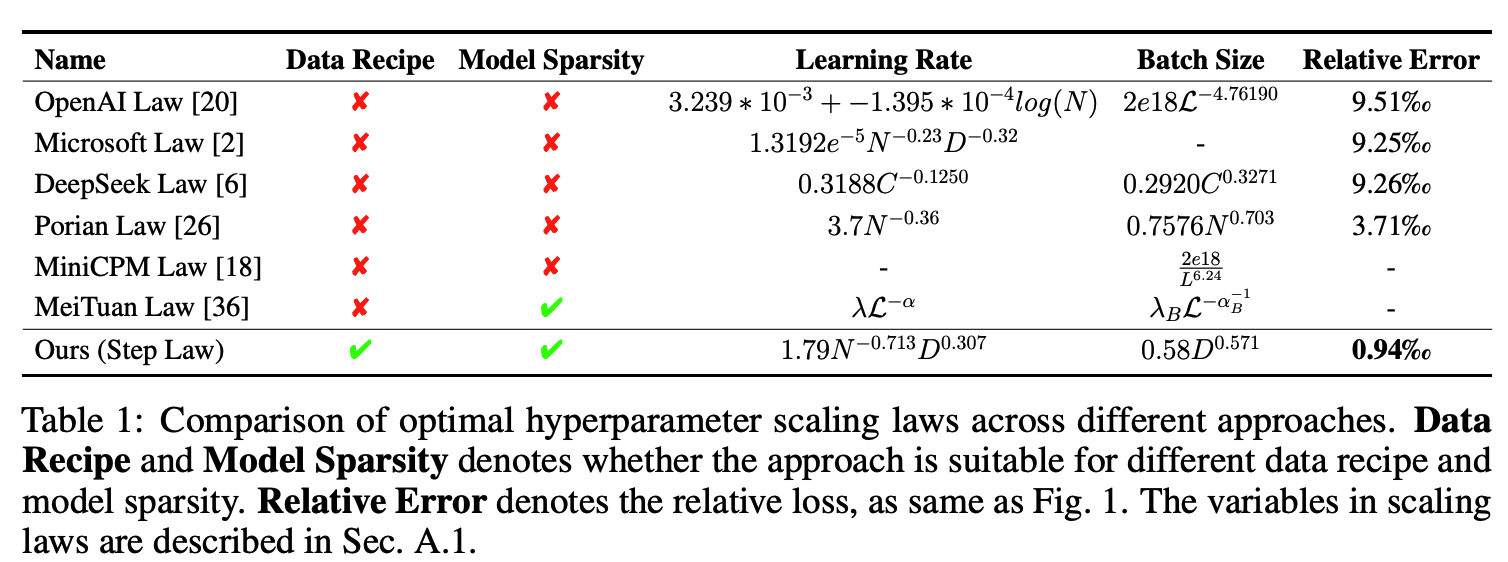
\includegraphics[width=0.95\linewidth,height=\textheight,keepaspectratio,alt={Step
Law 与已有超参数 Scaling Law 的对比}]{assets/steplaw-comparison.png}

\end{center}

\subsubsection{问题定义}\label{ux95eeux9898ux5b9aux4e49}

\begin{NotesFormula}

作者将最终训练损失表示为：

\[\mathcal L(\mathbb A,\mathbb D,N,D,\eta,B)\]

\end{NotesFormula}

其中：

\begin{itemize}
\tightlist
\item
  \(\mathbb A\)：模型架构。
\item
  \(\mathbb D\)：训练数据分布。
\item
  \(N\)：非 Embedding 参数量。
\item
  \(D\)：训练 Token 数。
\item
  \(\eta\)：Peak Learning Rate。
\item
  \(B\)：Token-wise Global Batch Size。
\end{itemize}

\begin{NotesFormula}

对于固定模型架构、数据分布以及训练规模，目标是：

\[(\eta^*,B^*)=\mathop{\arg\min}_{\eta,B}\,\mathcal L_{\mathbb A,\mathbb D,N,D}(\eta,B)\]

\end{NotesFormula}

\begin{NotesFormula}

进一步研究，是否存在仅依赖 \(N,D\) 的简单函数：

\[\boxed{\eta^*=f(N,D),\qquad B^*=g(N,D)}\]

\end{NotesFormula}

\subsubsection{实验规模}\label{ux5b9eux9a8cux89c4ux6a21}

\begin{itemize}
\tightlist
\item
  从头训练超过 3,700 个 LLM。
\item
  总计消耗约 100T Tokens。
\item
  使用接近 100 万 NVIDIA H800 GPU-hours。
\item
  系统性改变模型参数量、训练数据量、LR、BS、模型形状、MoE 稀疏度和 Data
  Recipe。
\end{itemize}

思路是：\textbf{先通过大规模 Grid Search
找到真实的最优超参数，再研究这些最优点如何随 \(N,D\)
变化，最终拟合具有预测能力的 Scaling Law。}

\subsubsection{Grid Search 设置}\label{grid-search-ux8bbeux7f6e}

超参数搜索主要采用对数间隔。

\begin{NotesFormula}

Learning Rate：

\[\eta_i=2^{-10.5+0.5i},\qquad i=0,\ldots,7\]

\end{NotesFormula}

\begin{NotesFormula}

Batch Size：

\[B_j=32768\cdot2^{j/2},\qquad j=0,\ldots,14\]

\end{NotesFormula}

因此：

\begin{itemize}
\tightlist
\item
  Learning Rate 共 8 个候选值。
\item
  Batch Size 共 15 个候选值。
\item
  完整的 \(8\times15\) Grid Search 包含 \textbf{120 组超参数组合}。
\end{itemize}

对于固定的 \(N,D\)，分别从头训练不同 LR、BS 的模型，记录最终的 Smoothed
Training Loss，确定 Loss 最小的超参数组合。

此外，Step 会\textbf{固定 End LR 为 1e-5}，而此前 DeepSeek 等工作通常将
End LR 设为 Peak LR 的固定比例（如 10\%）。但是如果 Peak 高的话也会带动
End 高，导致训到最后 Learning Rate 过高？那为什么不直接设置 End LR 为 0
呢？也许主要是为后面 Mid/Post Train 留下空间。

\subsubsection{Loss
Landscape：近似凸的碗形}\label{loss-landscapeux8fd1ux4f3cux51f8ux7684ux7897ux5f62}

\begin{center}

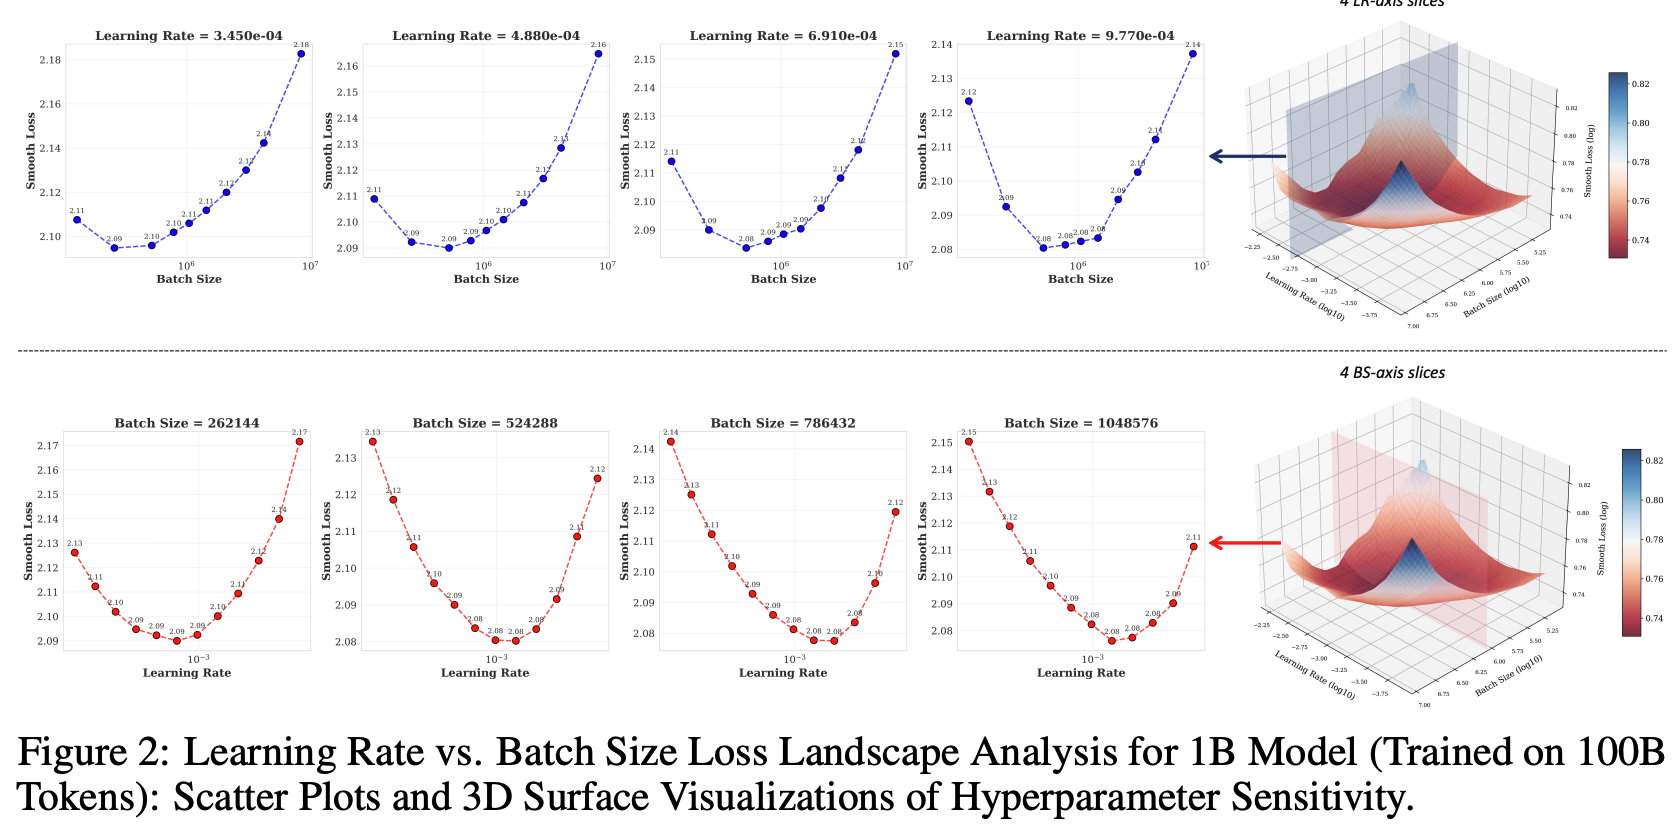
\includegraphics[width=0.95\linewidth,height=\textheight,keepaspectratio,alt={1B
模型（100B Tokens）的 LR--BS Loss
Landscape}]{assets/steplaw-landscape.png}

\end{center}

\begin{itemize}
\tightlist
\item
  LR 过小，参数更新不足，收敛缓慢。
\item
  LR 过大，训练容易不稳定。
\item
  BS 过小，梯度噪声较大。
\item
  BS 过大，给定 Token 预算下的优化步骤减少。
\end{itemize}

因此，Loss 在对数 LR--BS
空间中，通常表现出近似碗形的结构，存在一个较低的近似凸形的 Loss
Landscape。这点也让我们放点心：\textbf{预测精度不需要那么高，就可以接近最优的
Loss。}

\subsubsection{拟合 Step Law}\label{ux62dfux5408-step-law}

\begin{center}

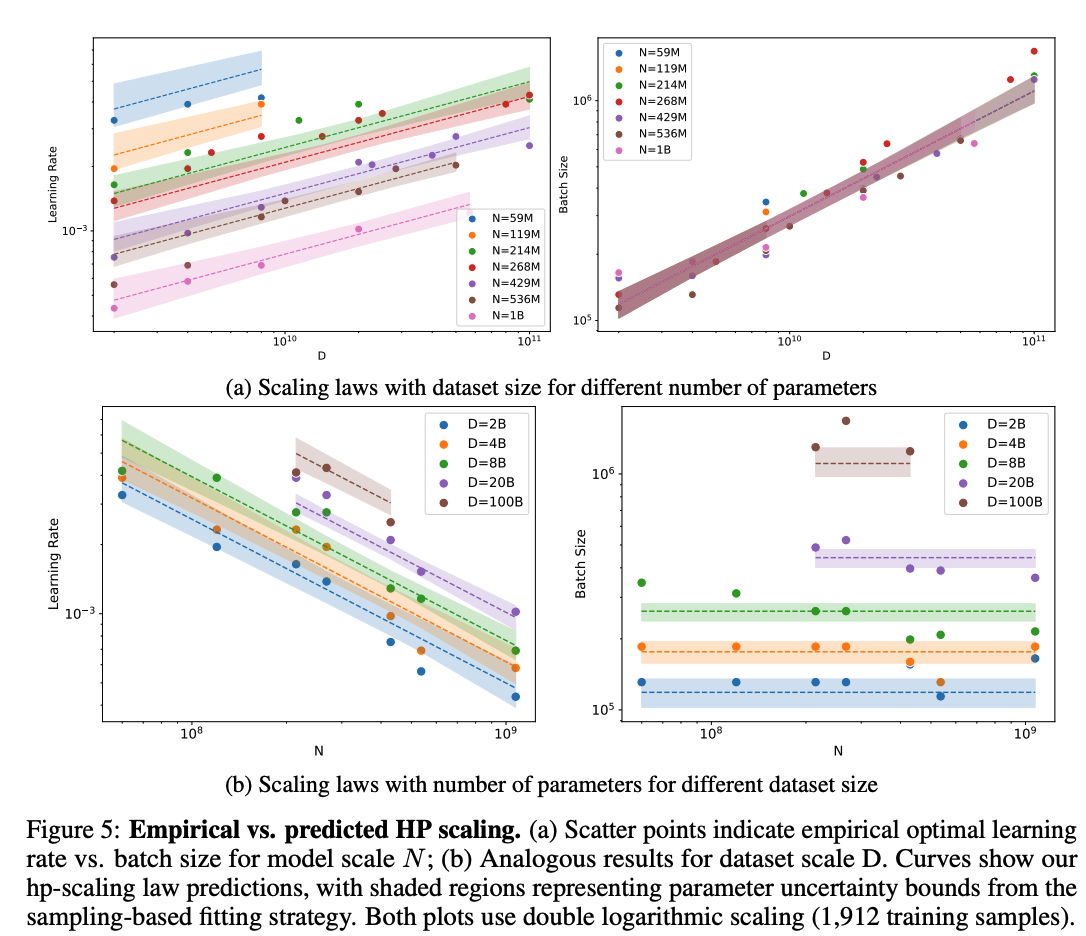
\includegraphics[width=0.88\linewidth,height=\textheight,keepaspectratio,alt={经验最优超参数与
Step Law 预测}]{assets/steplaw-fit.png}

\end{center}

观察最优超参数随 \(N,D\) 的变化趋势：

{\def\LTcaptype{none} % do not increment counter
\begin{longtable}[]{@{}
  >{\centering\arraybackslash}p{(\linewidth - 4\tabcolsep) * \real{0.2933}}
  >{\centering\arraybackslash}p{(\linewidth - 4\tabcolsep) * \real{0.3733}}
  >{\centering\arraybackslash}p{(\linewidth - 4\tabcolsep) * \real{0.3333}}@{}}
\toprule\noalign{}
\begin{minipage}[b]{\linewidth}\centering
\textbf{控制变量}
\end{minipage} & \begin{minipage}[b]{\linewidth}\centering
\textbf{最优 Learning Rate}
\end{minipage} & \begin{minipage}[b]{\linewidth}\centering
\textbf{最优 Batch Size}
\end{minipage} \\
\midrule\noalign{}
\endhead
\bottomrule\noalign{}
\endlastfoot
固定 \(N\)，增大 \(D\) & 增大 & 增大 \\
固定 \(D\)，增大 \(N\) & 减小 & 基本不变 \\
\end{longtable}
}

\begin{NotesFormula}

进一步在 Log-Log 坐标下观察，数据点呈现出近似线性关系。由于：

\[\log y=a\log x+b\iff y=e^bx^a\]

\end{NotesFormula}

\begin{NotesFormula}

因此，作者采用幂律形式：

\[\boxed{\eta(N,D)=cN^\alpha D^\beta},\qquad
\boxed{B(D)=dD^\gamma}\]

\end{NotesFormula}

其中 \(c,d,\alpha,\beta,\gamma\) 均为待拟合参数。

\begin{NotesFormula}

\textbf{Log-Linear Regression + Bootstrap}：首先，通过 Grid Search
获取不同模型规模 \(N\) 和训练数据量 \(D\) 下的最优 Learning Rate
\(\eta^*\) 和 Batch Size \(B^*\)；随后取对数，将幂律转化为线性关系，使用
OLS（普通最小二乘回归）拟合系数，即最小化预测值与实际最优超参数在 Log
空间中的平方误差。最后，通过 1000 次 Bootstrap
有放回重采样，重复拟合并统计系数分布，以估计参数的不确定性，最终得到：

\[\boxed{\eta^*=1.79N^{-0.713}D^{0.307},\qquad B^*=0.58D^{0.571}}\]

\end{NotesFormula}

\clearpage

\subsection{六、Farseer}\label{ux516dfarseer}

\textbf{Farseer: A Refined Scaling Law in Large Language Models}

Farseer 认为传统 Chinchilla Scaling Law 忽略了模型参数量 \(N\)
和训练数据量 \(D\) 之间的交互作用，因此提出一种新的 Loss Surface
\(L(N,D)\) 建模方法。其关键创新是\textbf{让数据 Scaling
的系数和指数都依赖于模型规模}，并利用 Differential Piecewise
Fitting（差分分阶段拟合）提高预测与外推精度。

\begin{itemize}
\tightlist
\item
  小模型容量有限，即使增加训练数据，也可能无法有效吸收更多知识。
\item
  大模型具有更强的表示能力，能够以不同的效率利用数据。
\item
  不同规模模型的数据 Scaling 曲线，其指数和系数可能同时发生变化。
\end{itemize}

\begin{NotesFormula}

从一般形式出发：

\[\boxed{L(N,D)=E+U(N)+V(D)+H(N,D)}\]

\end{NotesFormula}

相比 Chinchilla，额外引入
\(H(N,D)\)，表示参数规模与数据规模之间\textbf{无法通过两个独立函数加法分离的交互作用}。因此，研究的核心从拟合两个独立幂律，变成了寻找一个更准确、可外推的二维
Loss Surface。

不过，\(H(N,D)\)
无法直接从实验中独立观测，直接对四个函数分别拟合也比较困难。作者因此设计了一种\textbf{通过
Loss 差分消除无关项、逐步识别函数形式}的拟合方法。

\subsubsection{差分：消去不需要研究的项}\label{ux5deeux5206ux6d88ux53bbux4e0dux9700ux8981ux7814ux7a76ux7684ux9879}

\textbf{（1）固定模型规模 \(N\)，改变数据量 \(D\)}

\begin{NotesFormula}

定义：

\[\Delta_DL(N,D)=L(N,D)-L(N,\lambda D)\]

\end{NotesFormula}

\begin{NotesFormula}

展开：

\[\begin{aligned}
\Delta_DL(N,D)={}&V(D)-V(\lambda D)\\
&+H(N,D)-H(N,\lambda D)
\end{aligned}\]

\end{NotesFormula}

可以发现 \(E,\ U(N)\) 被完全消除。因此，\(\Delta_DL\)
只描述增加训练数据带来的 Loss 改善。

\begin{NotesFormula}

假设 Chinchilla 的独立加法形式成立：

\[\Delta_DL(N,D)=BD^{-\beta}(1-\lambda^{-\beta})\]

\end{NotesFormula}

此时该差分应当与 \(N\) 无关。但实验发现，\(\Delta_DL\) 不仅随 \(D\)
改变，也随 \(N\) 改变。这说明\textbf{数据 Scaling
规律具有模型规模依赖性}。

\textbf{（2）固定数据量 \(D\)，改变模型规模 \(N\)}

\begin{NotesFormula}

类似地：

\[\Delta_NL(N,D)=L(N,D)-L(\lambda N,D)\]

\end{NotesFormula}

\begin{NotesFormula}

展开：

\[\begin{aligned}
\Delta_NL(N,D)={}&U(N)-U(\lambda N)\\
&+H(N,D)-H(\lambda N,D)
\end{aligned}\]

\end{NotesFormula}

这次消除了 \(E\) 和
\(V(D)\)。如果模型参数量与数据量的作用完全可加分离，那么该差分不应依赖于
\(D\)。但实验同样发现了明显的数据规模依赖性。

\begin{center}

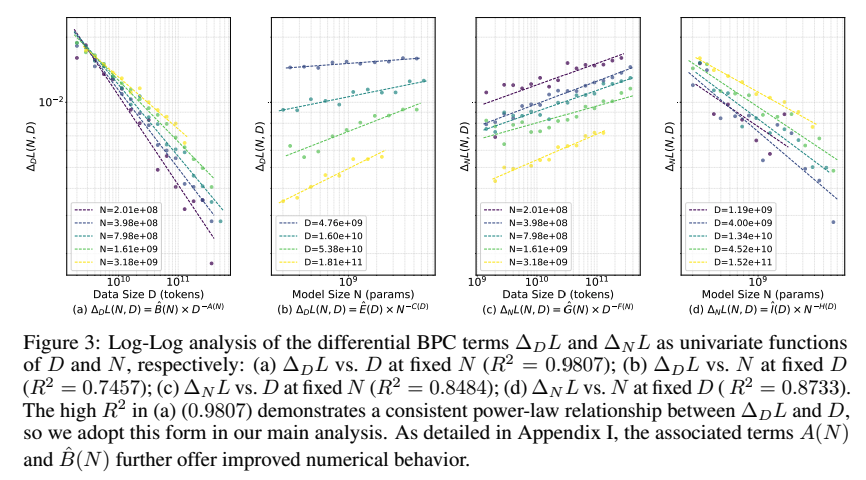
\includegraphics[width=0.95\linewidth,height=\textheight,keepaspectratio,alt={差分
BPC 项 \textbackslash Delta\_DL 与 D 的 Log-Log
分析}]{assets/farseer-differential.png}

\end{center}

\begin{NotesFormula}

论文发现固定 \(N\) 时，\(\Delta_DL\) 与 \(D\) 在 Log-Log
坐标系下近似线性（\(R^2=0.9807\)），因此假设：

\[\boxed{V(D)+H(N,D)\approx B(N)D^{-A(N)}}\]

\end{NotesFormula}

\subsubsection{Differential Piecewise
Fitting（差分分阶段拟合）}\label{differential-piecewise-fittingux5deeux5206ux5206ux9636ux6bb5ux62dfux5408}

\textbf{Stage 1：Differential + Log-Linear Regression}

\begin{NotesFormula}

固定模型规模 \(N\)，对不同数据量的 Loss 做差分，消除与 \(D\)
无关的模型规模项：

\[\begin{aligned}
R_N(D)&=L(N,D)-L(N,\lambda D)\\
&=B_N(1-\lambda^{-A_N})D^{-A_N}
\end{aligned}\]

\end{NotesFormula}

\begin{NotesFormula}

取对数：

\[\log R_N(D)=\log\hat B_N-A_N\log D\]

\end{NotesFormula}

通过线性回归，利用斜率和截距求出每个模型规模对应的 \(A_N,B_N\)，其中
\(\lambda=\sqrt2\)。

\textbf{Stage 2：Transformation Search + Iterative Fitting}

\begin{NotesFormula}

对 Stage 1 得到的离散 \(A_N,B_N\) 进行函数变换搜索，发现 Stretched
Exponential 拟合效果最好：

\[\boxed{
\begin{aligned}
A(N)&=\exp(a_1N^\alpha+b_1)\\
B(N)&=\exp(a_2N^\beta+b_2)
\end{aligned}}\]

\end{NotesFormula}

先通过 Grid Search + Linear Regression 确定参数，再交替优化
\(\alpha,\beta\)，最小化整体 Loss 差分的预测误差。

\textbf{Stage 3：Residual Fitting}

\begin{NotesFormula}

前两阶段只拟合了数据相关项
\(B(N)D^{-A(N)}\)，还需要拟合模型规模相关项。从原始 Loss
中减去数据相关项，并对不同 \(D\) 求平均：

\[G(N)=\operatorname{Avg}_D\left[L(N,D)-B(N)D^{-A(N)}\right]\]

\end{NotesFormula}

\begin{NotesFormula}

再次通过 Transformation Search，得到：

\[\boxed{G(N)=E+U(N)\approx\exp(a_3N^\gamma+b_3)}\]

\end{NotesFormula}

\begin{NotesFormula}

\textbf{最终 Scaling Law}

\[\boxed{L(N,D)=\exp(a_3N^\gamma+b_3)+\exp(a_2N^\beta+b_2)\,D^{-\exp(a_1N^\alpha+b_1)}}\]

\end{NotesFormula}

\begin{NotesFormula}

代入论文拟合的数值：

\[\boxed{
\begin{aligned}
L(N,D)={}&\exp\!\left(-0.021N^{0.169}-0.091\right)\\
&+\exp\!\left(88.01N^{-0.1}-6.287\right)\cdot D^{-\exp\left(-0.124N^{0.123}+0.424\right)}
\end{aligned}}\]

\end{NotesFormula}

这里 \(N\) 使用实际参数个数，\(D\) 使用实际 Token 个数，而不是直接以 B
为单位代入。

\textbf{核心优势}：将复杂的 9
参数非线性拟合拆解成多个更容易求解的一维问题，降低参数耦合与初始化敏感性。论文中，相比直接
Nonlinear Regression，拟合相对误差从 1.67\% 降至 0.18\%。

\clearpage

\subsection{七、MAI}\label{ux4e03mai}

\href{https://microsoft.ai/pdf/mai-thinking-1.pdf}{MAI Thinking
1}，\href{https://microsoft.ai/news/frontier-pre-training-at-microsoft-ai/}{Frontier
Pre-training at Microsoft AI}

\subsubsection{1. Scaling
Ladder（规模阶梯）}\label{scaling-ladderux89c4ux6a21ux9636ux68af}

构建一系列不同规模、遵循相同架构设计规则和训练 Recipe
的模型，用小模型实验指导大模型训练。

\begin{itemize}
\tightlist
\item
  每个模型以层数 \(L\) 定义规模，其他架构参数随 \(L\) 确定，例如
  \(d_{\mathrm{model}}=\frac{256}{3}L\)。
\item
  逐步训练 L18、L24、L30、L36、L42 等模型。
\item
  保持 TPP 不变，并通过 Source Scaling 控制数据重复次数。
\item
  利用小模型实验拟合 Scaling Law，预测最终 MAI-Base-2 的表现。
\end{itemize}

\begin{enumerate}
\def\labelenumi{\arabic{enumi}.}
\setcounter{enumi}{1}
\tightlist
\item
  Tokens per Active Parameter（TPP）
\end{enumerate}

\begin{NotesFormula}

定义为：

\[\boxed{TPP=\frac{D}{N_{\mathrm{active}}}}\]

\end{NotesFormula}

其中：

\begin{itemize}
\tightlist
\item
  \(D\)：训练过程中实际处理的总 Tokens，包含重复数据。
\item
  \(N_{\mathrm{active}}\)：每个 Token 激活的参数量。
\end{itemize}

\begin{NotesFormula}

MAI-Base-2：

\[TPP=\frac{50\mathrm{T}}{80\mathrm{B}}=625\]

\end{NotesFormula}

Scaling Ladder 中保持 TPP 固定，即模型激活参数量扩大多少倍，训练 Tokens
也扩大多少倍。

\textbf{核心目的}：控制不同规模模型的数据量与激活参数量之比，使不同规模实验具有可比性。

\subsubsection{3. Source
Scaling（数据源缩放）}\label{source-scalingux6570ux636eux6e90ux7f29ux653e}

\textbf{问题}：小模型训练 Horizon
较短，如果直接使用完整数据集，会导致小模型与大模型的数据重复次数不同，进而产生不同的过拟合压力。

\textbf{方法}：按比例缩小每个 Dataset
的唯一数据集合，使不同训练规模下，每个数据源的重复次数保持一致。例如，完整
50T 训练中，某数据源重复 8 次：

\begin{itemize}
\tightlist
\item
  大模型：使用完整唯一数据集，重复 8 次。
\item
  小模型：训练 Horizon 为 5T，只使用原数据集的 1/10，重复 8 次。
\end{itemize}

\begin{NotesFormula}

因此：

\[D'_{\mathrm{unique}}=\frac{D'_{\mathrm{train}}}{D_{\mathrm{train}}}D_{\mathrm{unique}}\]

\end{NotesFormula}

\begin{NotesFormula}

在固定 TPP 下：

\[\boxed{\frac{D'_{\mathrm{unique}}}{N'_{\mathrm{active}}}=\frac{D_{\mathrm{unique}}}{N_{\mathrm{active}}}}\]

\end{NotesFormula}

\textbf{核心目的}：同时保持数据重复次数和 Unique Data / Active
Parameters
的比例，避免小模型因重复数据不足而偏好正则化不足的架构和超参数。

\subsubsection{4. 如何预测最终
Loss？}\label{ux5982ux4f55ux9884ux6d4bux6700ux7ec8-loss}

\begin{enumerate}
\def\labelenumi{\arabic{enumi}.}
\tightlist
\item
  构建 Scaling Ladder，训练 L18--L42 等不同规模模型。
\item
  固定 TPP，使用 Source Scaling 控制数据重复次数。
\item
  记录各模型的训练 FLOPs 和 Held-out BPB。
\item
  拟合 BPB 与 Training FLOPs 之间的 Scaling Law。
\item
  将拟合曲线外推到目标模型 MAI-Base-2，预测最终 BPB。
\end{enumerate}

\begin{center}

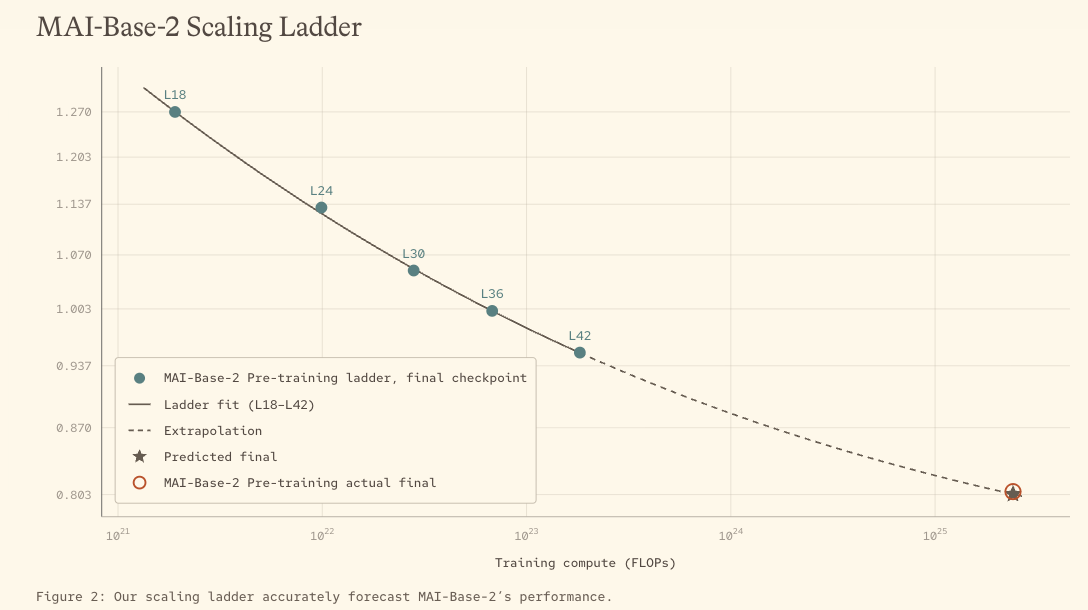
\includegraphics[width=0.88\linewidth,height=\textheight,keepaspectratio,alt={MAI-Base-2
Scaling Ladder}]{assets/mai-scaling-ladder.png}

\end{center}

\subsubsection{5. Efficiency
Gain（效率增益）}\label{efficiency-gainux6548ux7387ux589eux76ca}

\textbf{问题}：直接比较两个模型的 Loss，会混淆模型规模、训练计算量和训练
Recipe 的影响。

\textbf{方法}：在相同评测 Loss 下，比较两个模型分别需要多少计算资源。

\begin{itemize}
\tightlist
\item
  \(EG_{\mathrm{FLOPs}}\)：相同 Loss 下所需 FLOPs
  的效率倍数，衡量算法和模型设计的计算效率。
\item
  \(EG_{\mathrm{time}}\)：相同 Loss 下所需 Wall-clock Time
  的效率倍数，衡量实际训练时间效率，包含系统实现和硬件利用率的影响。
\end{itemize}

\begin{NotesFormula}

直观上，效率倍数可以理解为：

\[EG=\frac{C_{\mathrm{baseline}}}{C_{\mathrm{candidate}}}\]

\end{NotesFormula}

其中 \(C\) 表示达到相同 Loss 所需的计算量。微软主要关注
\(EG_{\mathrm{time}}\)，因为实际训练成本取决于真实运行效率。

\begin{NotesFormula}

\textbf{实验结果}：对四个 Held-out 评测集分别拟合 BPB--FLOPs Scaling
Law，反推出 MAI Recipe 达到 DeepSeek-V4-Pro-Base 相同 BPB
所需的计算量。MAI-Base-2 相比 DeepSeek-V4-Pro-Base：

\[\boxed{EG_{\mathrm{FLOPs}}=4.2\sim12.3\times}\]

\end{NotesFormula}

当然，这个数字因为很难做到完全公平肯定会有偏向MAI的程度，loss
也并不能完全反应模型能力。

\subsubsection{6. Hyperparameter Scaling
Laws（超参数缩放定律）}\label{hyperparameter-scaling-lawsux8d85ux53c2ux6570ux7f29ux653eux5b9aux5f8b}

\textbf{研究目标}：Again，利用小模型实验，预测大规模预训练所需的最优
LR、WD 和 Dropout，减少大模型超参数搜索成本。

\textbf{（1）LR 与 WD 联合搜索}

\begin{NotesFormula}

作者发现 LR 和 WD 存在明显耦合关系，模型表现对 \(LR\times WD\)
尤其敏感。因此不直接在 \((\log LR,\log WD)\) 上做二维网格搜索，而是在：

\[\boxed{(\log LR,\ \log(LR\times WD))}\]

\end{NotesFormula}

上联合搜索。

\textbf{（2）二维二次曲面拟合}

\begin{NotesFormula}

对不同模型规模和 TPP 的实验结果，拟合：

\[\mathcal L(x,y)=ax^2+by^2+cxy+dx+ey+f,\qquad
x=\log LR,\quad y=\log(LR\times WD)\]

\end{NotesFormula}

通过求解曲面的解析最小值，得到最优 \((LR^*,\ LR^*\times WD^*)\)。

\textbf{（3）拟合 Hyperparameter Scaling Laws}

\begin{NotesFormula}

通过不同模型规模、TPP 和训练 Steps 下的最优超参数，拟合得到：

\[\boxed{LR^*\times WD^*=\frac{17.04}{S}},\qquad
\boxed{\log LR^*=-1.51+0.175\log TPP-0.573\log S}\]

\end{NotesFormula}

其中 \(S\) 是训练总 Steps。由此可以得到：

\begin{itemize}
\tightlist
\item
  \(LR^*\times WD^*\propto S^{-1}\)：训练步数越多，LR 与 WD 的乘积越小。
\item
  \(LR^*\propto S^{-0.573}\)：训练步数越多，最优 LR 越小。
\item
  \(LR^*\propto TPP^{0.175}\)：固定训练步数时，TPP 越大，最优 LR 越大。
\end{itemize}

\clearpage

\subsection{八、最优 LR
规律对比}\label{ux516bux6700ux4f18-lr-ux89c4ux5f8bux5bf9ux6bd4}

前面几章都给出了最优 LR 的 Scaling
Law，但结论乍看互相矛盾：同样是训练数据量 \(D\) 增大，Microsoft Law
认为最优 LR 下降，Step Law 却认为上升。

{\def\LTcaptype{none} % do not increment counter
\begin{longtable}[]{@{}
  >{\centering\arraybackslash}p{(\linewidth - 6\tabcolsep) * \real{0.1840}}
  >{\centering\arraybackslash}p{(\linewidth - 6\tabcolsep) * \real{0.3280}}
  >{\centering\arraybackslash}p{(\linewidth - 6\tabcolsep) * \real{0.2960}}
  >{\centering\arraybackslash}p{(\linewidth - 6\tabcolsep) * \real{0.1920}}@{}}
\toprule\noalign{}
\begin{minipage}[b]{\linewidth}\centering
\textbf{工作}
\end{minipage} & \begin{minipage}[b]{\linewidth}\centering
\textbf{最优 LR 规律}
\end{minipage} & \begin{minipage}[b]{\linewidth}\centering
\textbf{Batch Size}
\end{minipage} & \begin{minipage}[b]{\linewidth}\centering
\textbf{实验条件}
\end{minipage} \\
\midrule\noalign{}
\endhead
\bottomrule\noalign{}
\endlastfoot
\textbf{DeepSeek LLM} & \(\eta_{\mathrm{opt}}\propto C^{-0.125}\) &
\(B_{\mathrm{opt}}\propto C^{0.327}\) & 以算力 \(C\) 为自变量 \\
\textbf{Microsoft Law} & \(\eta^*\propto N^{-0.23}D^{-0.32}\) & 固定
0.5M Tokens & 只改变 \(D\)，BS 不变 \\
\textbf{Step Law} & \(\eta^*\propto N^{-0.713}D^{+0.307}\) &
\(B^*\propto D^{0.571}\) & LR 与 BS 同时取最优 \\
\textbf{MAI} & \(LR^*\propto TPP^{0.175}\,S^{-0.573}\) & --- & 把 TPP
与步数 \(S\) 分开 \\
\end{longtable}
}

\textbf{矛盾来自 Batch Size 是否随 \(D\) 变化。} 训练步数
\(S=D/B\)，而最优 LR 主要由步数决定：

\begin{itemize}
\tightlist
\item
  \textbf{Microsoft Law}：\(B\)
  固定，\(S\propto D\)，步数随数据量线性增加，最优 LR 下降。
\item
  \textbf{Step Law}：\(B^*\propto D^{0.571}\)，步数只按
  \(S\propto D^{0.429}\) 增长；Batch 变大、梯度噪声变小，又允许更大的
  LR，两者综合后最优 LR 反而上升。
\item
  \textbf{DeepSeek}：同理，算力增加时最优 BS 随之增大，最优 LR
  只缓慢下降（指数仅 \(-0.125\)）。
\end{itemize}

\textbf{MAI 的形式把两种效应拆开了}：步数越多，最优 LR
越小（\(S^{-0.573}\)）；固定步数时，每个参数见到的 Token 越多（等价于
Batch 越大），最优 LR 越大（\(TPP^{0.175}\)）。粗略代入 Microsoft Law
的设置（固定 \(N\) 与 \(B\)，则 \(TPP\propto D\)，\(S\propto D\)），得到
\(LR^*\propto D^{0.175-0.573}=D^{-0.40}\)，与 Microsoft Law 的
\(D^{-0.32}\) 量级相近。

\textbf{参考资料}

{[}1{]} Rosenfeld et al.：\href{https://arxiv.org/abs/1909.12673}{A
Constructive Prediction of the Generalization Error Across Scales}

{[}2{]} Kaplan et al.：\href{https://arxiv.org/abs/2001.08361}{Scaling
Laws for Neural Language Models}

{[}3{]} Hoffmann et
al.：\href{https://arxiv.org/abs/2203.15556}{Training Compute-Optimal
Large Language Models}

{[}4{]} DeepSeek-AI：\href{https://arxiv.org/abs/2401.02954}{DeepSeek
LLM: Scaling Open-Source Language Models with Longtermism}

{[}5{]} Besiroglu et
al.：\href{https://arxiv.org/abs/2404.10102}{Chinchilla Scaling: A
replication attempt}

{[}6{]} Bjorck et al.：\href{https://arxiv.org/abs/2409.19913}{Scaling
Optimal LR Across Token Horizons}

{[}7{]} StepFun：\href{https://arxiv.org/abs/2503.04715}{Predictable
Scale: Part I, Step Law -- Optimal Hyperparameter Scaling Law in Large
Language Model Pretraining}

{[}8{]} Li et al.：\href{https://arxiv.org/abs/2506.10972}{Predictable
Scale: Part II, Farseer: A Refined Scaling Law in Large Language Models}

{[}9{]} Lilian
Weng：\href{https://lilianweng.github.io/posts/2026-06-24-scaling-laws/}{Scaling
Laws}

{[}10{]} 苏剑林：\href{https://kexue.fm/archives/11833}{解构Scaling
Law：优化、架构、数据的三重奏}

{[}11{]} Stanford CS336：Lecture 09、Lecture 11（Scaling Laws）

{[}12{]} Microsoft
AI：\href{https://microsoft.ai/pdf/mai-thinking-1.pdf}{MAI Thinking 1}

{[}13{]} Microsoft
AI：\href{https://microsoft.ai/news/frontier-pre-training-at-microsoft-ai/}{Frontier
Pre-training at Microsoft AI}

\end{document}
